\documentclass[../../main.tex]{subfiles}

\begin{document}
    
\section{Images}
Images are likely to be chosen to hide secret messages due to the low
sensibility of the \emph{human visual system} (HVS) to some particular
attributes such as small changes in luminance or brightness or contrast near
figures edges.
There are several methods to apply steganography to an image, in the
following sections we will treat some of the most common hiding techniques
and some of the steganalysis methods to deal with them.

\subsection{Stego-key search and encryption}

It is important to notice that when we refer to modifications of the \emph{LSB} in images we
do not necessarily imply modifications to every byte. Whenever allowed by the size of the cover type, it is 
more useful and dicrete to follow some pseudo-random sequence. This sequence is usually decided by a \emph{stego-key} (usually stego-key will be mapped in a set of possible
seeds by a hash map) \cite{stego-key}.

We also want to point out that the embedding of information could also be preceded by an encryption of such information.
This procedure makes the extraction of the message through a brute fore approce practically unfeasible: the complexity would
be proportional to the cardinality of the set of possible seeds time the
one of the set of possible encryptions. Although the encrypted message is still susceptible to attacks.

\subsection{LSB embedding method}
LSB embedding method is arguably the most popular steganographic method, due
to its simplicity, high imperceptibility and high capacity.
In this method, the image is decomposed into \emph{bits plane} (8 bits per
pixel for grayscale and 24 for color images, one for each color channel)
and the \emph{least significant bit} (LSB) is substituted with the message
to be hidden.
Note that even if the message is encrypted, due to its simplicity, this
method is easily detectable with a statistical steganalysis attack
\cite{techniques-data-hiding}.

\subsection{Difference Image Histogram method}
The \emph{Difference Image Histogram method} is derived by the easier idea
of analysing the \emph{histogram distribution} of a natural image and its
stegoimage. When we are steganalysing an image we usually do not
have the cover image. What we can do is comparing the histogram
distribution of the stegoimage with a set of images similar to the one. 
By the law of large numbers we should be able to find a \emph{mean imgae} to use to compare with our stegoimage.
The criticalities arise when the set is polluted.
\cite{methodology-steganalysis-images}

The proposed way to proceed is the following
\cite{new-detection-lsb-steganography}. 
Starting from the test image (that we will call $h$, considering $h$ a grayscale image or a color image under
some assumptions) we initially generate an image $f$ given by $h$ with flipped LSB. 
Then an image $g$ given by $h$ zeroing the LSB. Finally images $D_h$, $D_f$, $D_g$, 
created by the respective image of each one with the following formula:
          \[ D_{I}(i,j) = I(i+1,j) - I(i,j) \]
where $I$ is the image denoted by the subscript and the couple and
$(i,j)$ a unique pixel of the image.
At this point, we can analyse the histograms of the three generated images
$D_h$, $D_f$, $D_g$:
\[
    H = \{h_i | i = -255,\ ...,\ +255\},\ 
    F = \{f_i | i = -255,\ ...,\ +255\},\ 
    G = \{g_i | i = -255,\ ...,\ +255\}
\]

\begin{figure}[h]
    \centering
    \caption{Transition values from $G$ to $H$ and $F$}
    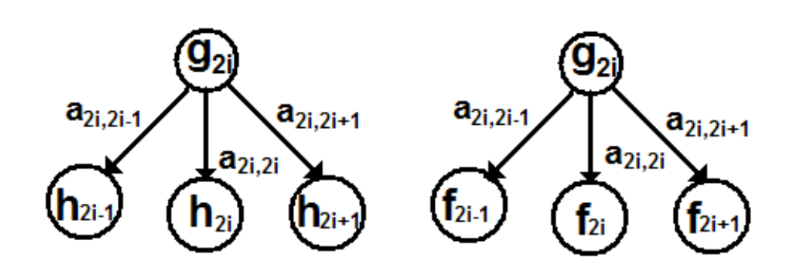
\includegraphics[scale=0.4]{difference_histogram_mtd.png}
\end{figure}

then, we define the following values: $\alpha_i = \frac{a_{2i+2,2i+1}}{a_{2i,2i+1}}$ $ \beta_i = \frac{a_{2i+2,2i+3}}{a_{2i,2i-1}}$ $\gamma_i = \frac{g_{2i}}{g_{2i+2}}$


As described by X. Ping and T. Zhang in
\cite{new-detection-lsb-steganography}:
\begin{itemize}[noitemsep]
    \item if $\alpha_i \approx 1, \forall i \in \{-255, -254, ..., 255\}$
          then the image contains some hidden message;
    \item otherwise, for natural images, $\alpha_i \approx \gamma_i$ is
          satisfied.
\end{itemize}

\subsection{Closest Color Pair method}
Another method used to detect hidden messages on the LSB plane is the
\emph{Closest Color Pair method}.

When an image has a steganographed message in te LSB plane, the number of
close colors increases \cite{detecting-lsb-steganography}. Given two pair of
colors $C_1=[R_1,G_1,B_1],\ C_2=[R_2,G_2,B_2]$, the condition of them being
close is:

\[ (R_1-R_2)^2+(G_1-G_2)^2+(B_1-B_2)^2 \leq 3 \]

We apply a LSB embedding steganography algorithm on the image and we compute
the number of close color pairs in both images.

Now, we define:

\begin{itemize}[noitemsep]
    \item $P$ as the number of close color pairs; $P'$ as the number of
          close color pairs of the stegoimage;
    \item $U$ as the number of color pairs; $U'$ as the number of color
          pairs of the stegoimage
\end{itemize}

Then, we compute:

\[ R = \frac{P}{\binom{U}{2}},\ R' = \frac{P'}{\binom{U'}{2}} \]

We know that if

\[ \frac{R}{R'} \geq Th,\ Th = 1.1 \]

\noindent then the image is a natural image, otherwise it contains an hidden
message. All the proofs are in \cite{detecting-lsb-steganography}.

\subsection{JPEG steganalysis}
JPEG images are one of the most used format on Internet web sites, due to
their high compression rate, while maintaining a good quality.
\subsubsection{DCT Domain embedding methods}
The DCT Domain embedding methods modify the compression coefficients
in order to hide data inside the image.
The JPEG format uses a \emph{discrete cosine transform} (DCT) to transform
every 8x8-pixel block into 64 DCT coefficients, that are used to calculate
the pixels when the image is displayed.
The simplest and most used DCT Domain embedding method substitute the
\emph{LSB} of the coefficients with the secret message: since the
modification is done in the frequency domain, there is no human perceivable
change in the image.
However, these modifications can be detected by analyzing the DCT coefficients
which changes significantly with respect to a natural image
\cite{jpeg-image-internet}.
\subsubsection{Chi-square test}
The Chi-square test is a statistical steganalysis test, which aims
at determining whether an image shows distorsion from embedding hidden data.\\
Let $n_i$ be the frequency of the DCT coefficient $i$ in the
image, we assume that an image with hidden data has similar
frequency for adjacent coefficients so we compute the arithmetic
mean $y_{i}^{*} = \frac{n_{2i}+n_{2i+1}}{2}$ to derive the expected
distribution.\\
The expected distribution is compared with the observed one $y_i = n_{2i}$.\\
The chi-square distribution for the difference between the
expected and the observed DCT coefficients is calculated as follows:
$$ \chi^2 = \sum_{i=1}^{\nu+1}
\frac{\left( y_i-y_{i}^{*}\right)}{y_{i}^{*}}$$
where $\nu$ are the degrees of freedom, which are one less than the categories in the DCT coefficients histogram.\\
The probability that there is an embedded message can be computed
as the complement of the \emph{cumulative distribution function} of
the chi-square distribution.\\

Note that, as presented in the stego-key section, different algorithms
modify the coefficients not sequentially or following different orders, so
the steganalysis process is usually performed by calculating the probability
of the presence of an embedded message considering different portions of the
image at the same time \cite{jpeg-image-internet}.

\end{document}